\documentclass[professionalfonts,aspectratio=169]{beamer}

\usetheme{Madrid}
%  Section created with help of AI
\setbeamertemplate{footline}{
  \leavevmode%
  \hbox{%
  \begin{beamercolorbox}[wd=.25\paperwidth,ht=2.5ex,dp=1ex,left]{author in head/foot}%
    \hspace{1em}Valentin Levchenko (Master CSMI)
  \end{beamercolorbox}%
  \begin{beamercolorbox}[wd=.5\paperwidth,ht=2.5ex,dp=1ex,center]{title in head/foot}%
    Statistical Characterisation of High-Field Magnet Operations
  \end{beamercolorbox}%
  \begin{beamercolorbox}[wd=.25\paperwidth,ht=2.5ex,dp=1ex,right]{date in head/foot}%
    \insertframenumber{} / \inserttotalframenumber \hspace{1em}
  \end{beamercolorbox}}%
}
%  Section created with help of AI

\usecolortheme{default}

\usepackage[english]{babel}
\usepackage{amsmath,amssymb}
\usepackage{graphicx}
\usepackage{booktabs}
\usepackage{hyperref}
\usepackage{listings}
\usepackage{color}

\lstset{language = Python,
        basicstyle = \ttfamily\small,
        keywordstyle = \color{blue},
        commentstyle = \color{gray},
        showstringspaces = false,
        breaklines = true}


%=============================================================================================


\setbeamersize{text margin left=5mm, text margin right=5mm}
\sloppy
\emergencystretch=3em

\title{Stage: Statistical Characterisation of High-Field Magnet Operations}
\author{Valentin Levchenko\\[0.3 cm]
        \footnotesize \textbf{Supervisors}: Christophe Trophime, Joubine Aghili}
\institute{Master CSMI \\
           University of Strasbourg \\[0.1 cm]
           Laboratoire National des Champs Magnétiques Intenses \\[0.1 cm]
           Centre National de la Recherche Scientifique}
\date{Academic Year 2025--2026}


%=============================================================================================


\begin{document}

\begin{frame}
    \titlepage
\end{frame}

\addtobeamertemplate{footline}{}{%
    \begin{beamercolorbox}[wd=\paperwidth,ht=2.5ex,dp=1.2ex,leftskip=1em]{author in head/foot}
        \usebeamerfont{author in head/foot}
        Master CSMI -- University of Strasbourg
    \end{beamercolorbox}
}


%=============================================================================================


\begin{frame}{Context}
    \begin{itemize}

        \item \textbf{CNRS} (Centre National de la Recherche Scientifique) \cite{lncmi}
        \begin{itemize}
            \item Largest public research organisation in France
        \end{itemize}

        \item \textbf{LNCMI} (Laboratoire National des Champs Magnétiques Intenses)
        \begin{itemize}
            \item National facility for high magnetic field research
            \item Based in Grenoble \& Toulouse
            \item Member of \textbf{EMFL} (European Magnetic Field Laboratory)
            \begin{itemize}
                \item Provides access to high-field facilities
            \end{itemize}
        \end{itemize}
        
        
    \end{itemize}
\end{frame}

%---------------------------------------------------------------------------------------------

\begin{frame}{Objectives}
    \begin{itemize}
        \item Organise experimental records from LNCMI magnets 
        \item Build a unified database of experiment files
        \item Compute operational indicators from magnet runs
        \item Develop tools for data exploration and monitoring
    \end{itemize}
\end{frame}

%---------------------------------------------------------------------------------------------

\begin{frame}{Work Completed Last Week}
    \begin{itemize}
        \item Installed and validated MagnetDB analysis tools
        \item Prepared local copies of experimental records
        \item Studied the structure of magnet experiment data
        \item Developed an initial dashboard for experiment exploration
    \end{itemize}
\end{frame}

%---------------------------------------------------------------------------------------------

\begin{frame}{Environment Setup}
    \begin{itemize}
        \item Built a Docker-based development environment
        \item Installed:
        \begin{itemize}
            \item python\_magnetrun
            \item python\_magnetgeo
            \item python\_magnetcooling
        \end{itemize}
        \item Resolved Git submodule issues
        \item Created isolated Python virtual environment
    \end{itemize}
\end{frame}

%---------------------------------------------------------------------------------------------

\begin{frame}{Dataset Preparation}
    \begin{itemize}
        \item Imported experimental Pupitre archives
        \item Organised local storage of experimental files:
        \begin{itemize}
            \item \texttt{\~/LNCMIG-Data/records}
        \end{itemize}
        \item Verified compatibility with MagnetDB workflows
        \item Prepared datasets for statistical processing
    \end{itemize}
\end{frame}

%---------------------------------------------------------------------------------------------

\begin{frame}{Operational Statistics}
    \begin{itemize}
        \item For each run, several indicators are computed:
        \begin{itemize}
            \item Total experiment duration:
            \[
            T_{\mathrm{run}} = \sum_i \Delta t_i
            \]
            \item Time spent above magnetic field threshold
            \[
            T_{\mathrm{field}} = \sum_{B_i > B_{\mathrm{th}}}\Delta t_i
            \]
            \item Electrical energy consumption
            \[
            E_{\mathrm{elec}} = \sum_i P_{\mathrm{tot}, i}\,\Delta t_i
            \]
        \end{itemize}
    \end{itemize}
\end{frame}

%---------------------------------------------------------------------------------------------

\begin{frame}{Operational Statistics}
    \begin{itemize}
        \item For each run, several indicators are computed:
        \begin{itemize}
            \item Estimated extracted thermal energy
            \[
            E_{\mathrm{thermal}} = \sum_i (T_{sb, i} - T_{eb, i})\,Q_i\,\rho c_p\,\Delta t_i
            \]
            where
            \begin{itemize}
                \item $T_{eb}$: inlet water temperature
                \item $T_{sb}$: outlet water temperature
                \item $Q$: water flow rate
                \item $\rho$: water density
                \item $c_p$: specific heat capacity
            \end{itemize}
        \end{itemize}
    \end{itemize}
\end{frame}

%---------------------------------------------------------------------------------------------

\begin{frame}{Dashboard}
    \centering
    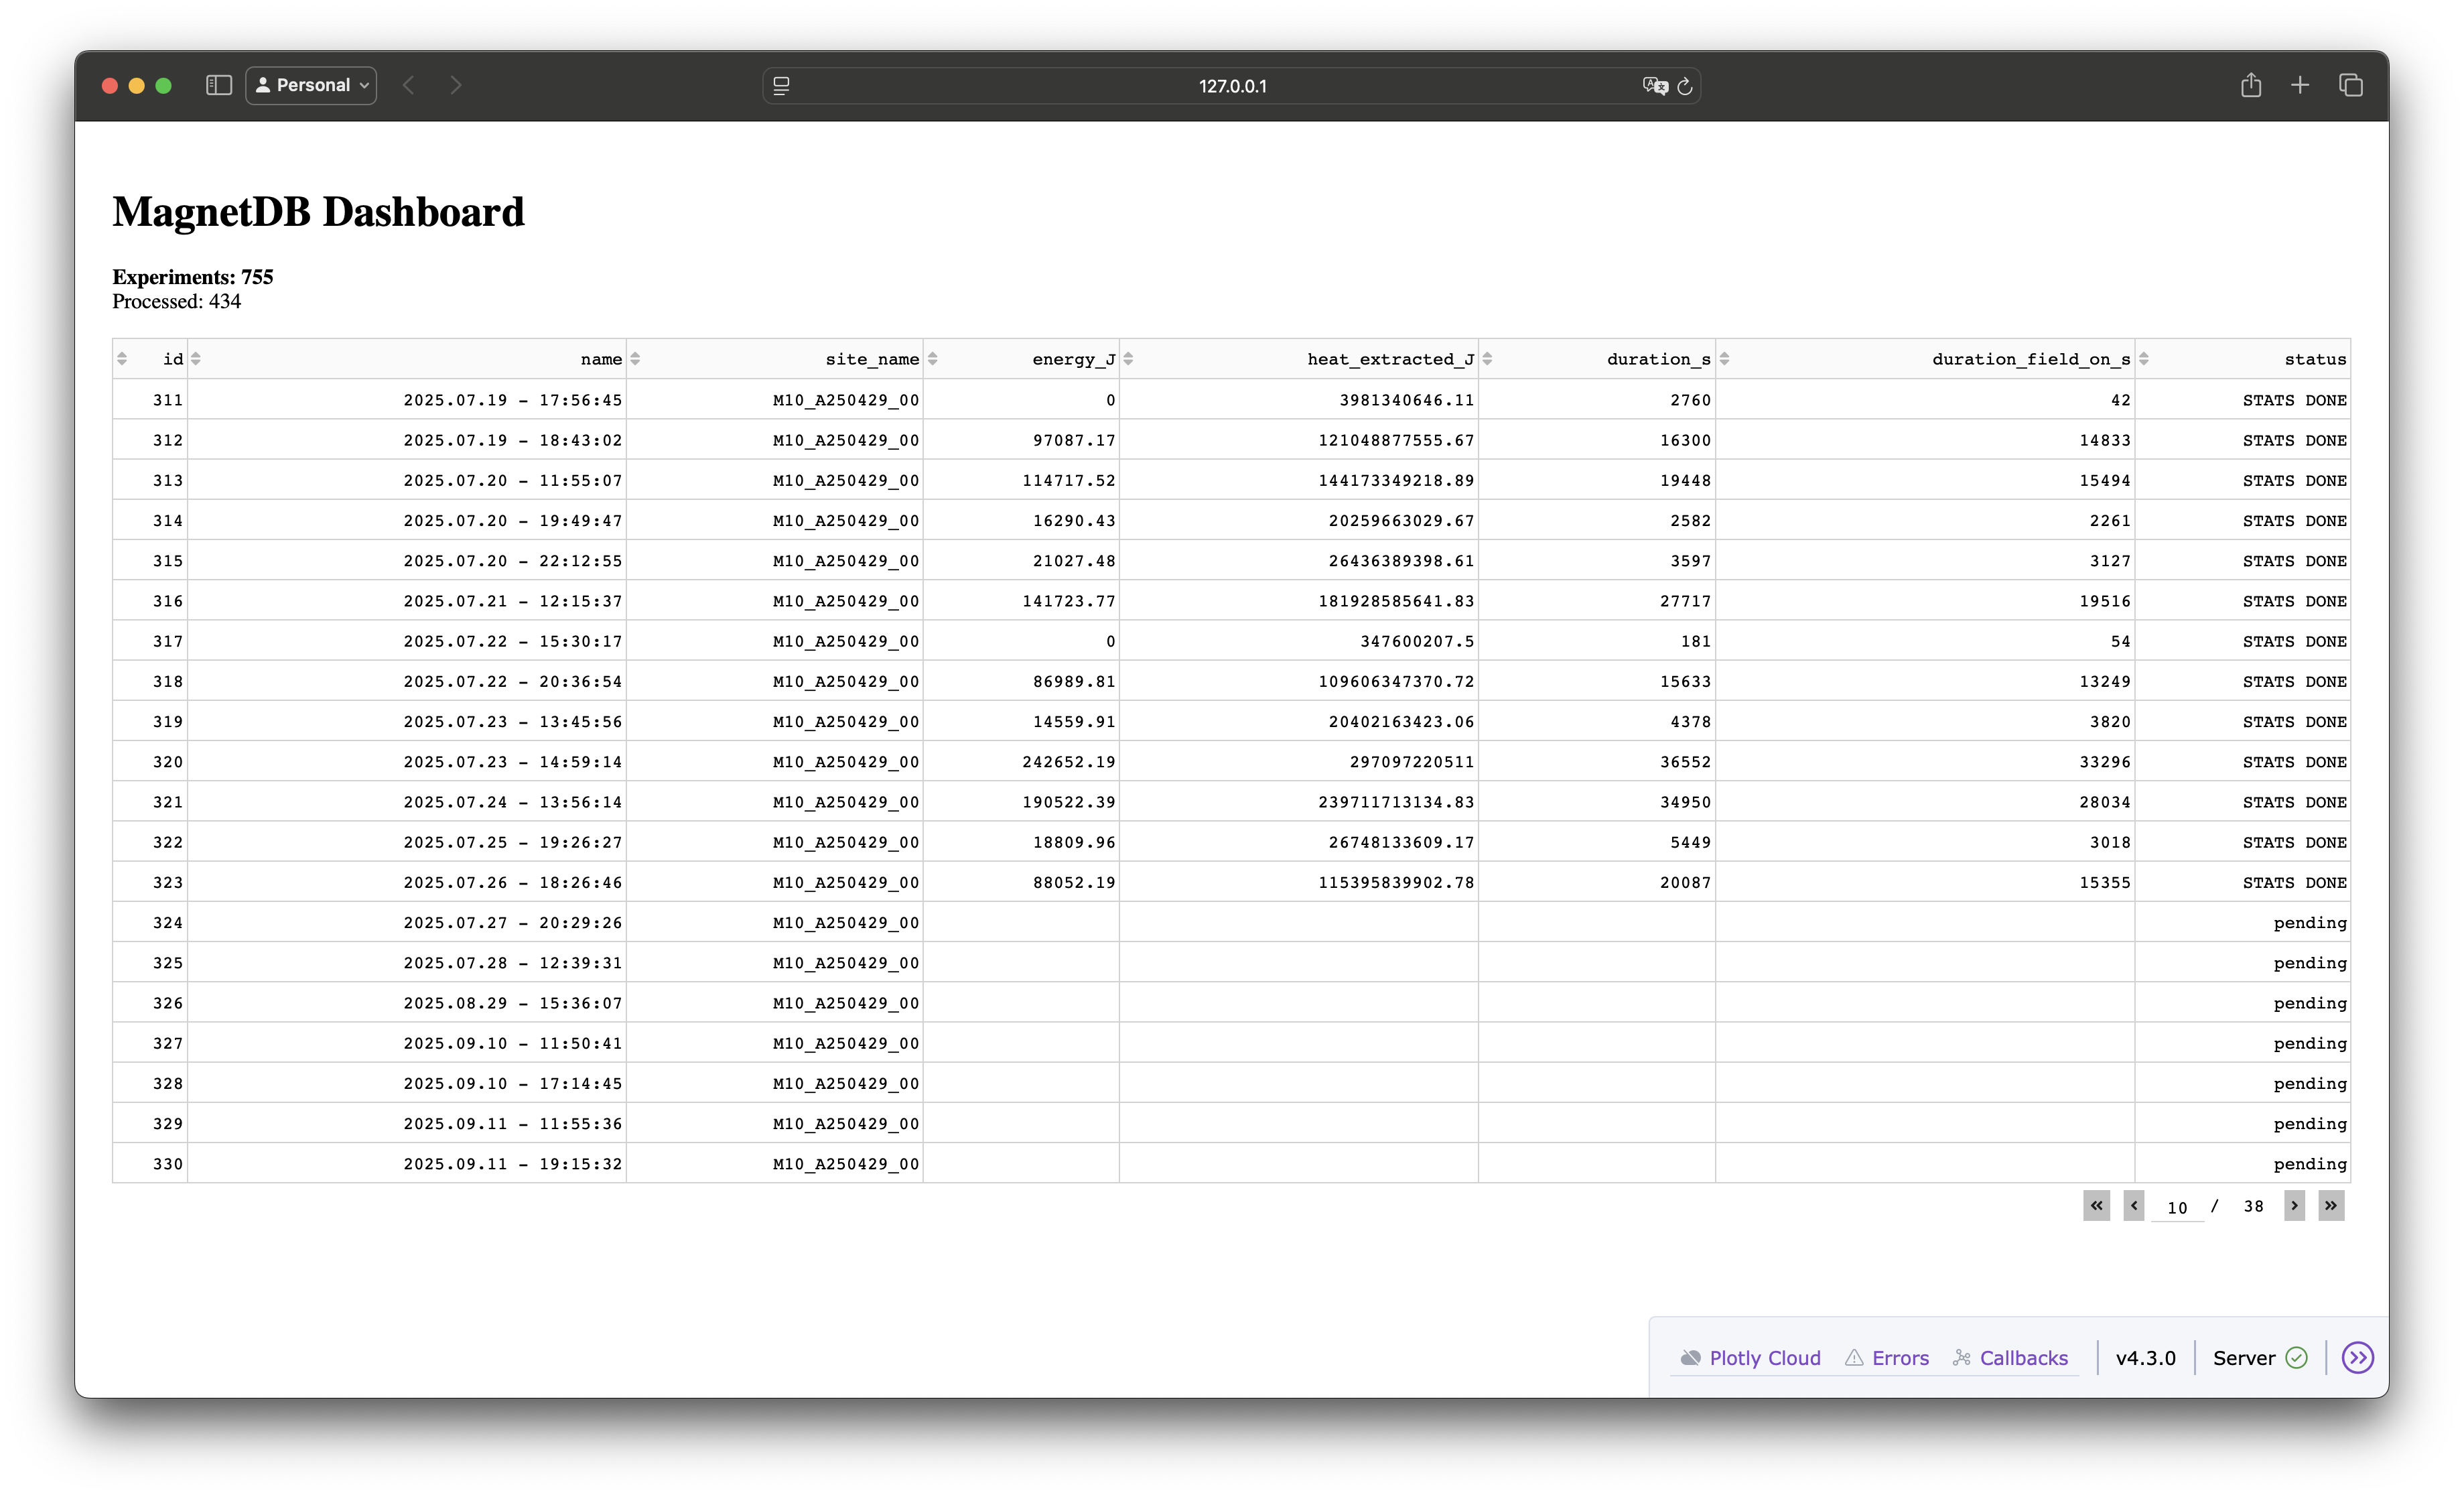
\includegraphics[width=\textwidth]{dashboard.png}
\end{frame}

%---------------------------------------------------------------------------------------------

\begin{frame}{Current Status}
    \begin{itemize}
        \item Experimental datasets available locally
        \item MagnetDB Python tools operational
        \item Statistics computation pipeline validated
        \item Dashboard connected to experiment records
        \item Ready for large-scale statistical processing
    \end{itemize}
\end{frame}

%---------------------------------------------------------------------------------------------

\begin{frame}{Possible Future Work}
    \begin{itemize}
        \item Complete integration of experimental statistics into MagnetDB workflows
        \item Automatic computation of statistics for newly imported experiment files
        \item Secondary database to store processing results without modifying the original database
    \end{itemize}
\end{frame}

%=============================================================================================

\iffalse
\begin{frame}{References}
    \bibliographystyle{unsrt}
    \bibliography{references}
\end{frame}
\fi

%=============================================================================================

\end{document}